\section{Evaluation Framework}
\label{sec:evaluation}
%%
This section describes the evaluation data and methodology.
%% This section describes the data used and the experimental methodology adopted for evaluating the proposed file recommendation system. 

\subsection{Data}
\label{sec:data}
\begin{table*}[!htpb]
\centering
\caption{Statistics of shares used for evaluation } 
{\fontsize{8pt}{1em}\selectfont
%\begin{tabular}{|p{0.5cm}|p{1.28cm}|r|p{1.15cm}|p{1.1cm}|p{1.4cm}|}
  %\begin{tabular}{|>{\centering}p{0.8cm}|r|r|>{\centering}p{2.7cm}|>{\centering}p{2.3cm}|r|}
\begin{tabular}{|>{\centering}p{0.8cm}|r|r|r|r|r|}
\hline
%Share & Sample period (days) & Users & Files operated on & Total file operations &Norm. Triangle Count \\
\textbf{Share} & \textbf{\# days} & \textbf{\# users} & \textbf{\# files operated on} & \textbf{\# file operations} &\textbf{Norm. Triangle Count} \\
\hline
A & 123 & 992 & 36,009 & 11M &  8K \\ \hline
B & 122 & 464 & 1,309 & 136K &3K \\ \hline%Correction made to camera ready
C & 122 & 160 & 1,044,779 & 3M &  $<$0.1\\ \hline
D & 121 & 183 & 746 & 11K & 951\\ \hline%Correction made to camera ready
E & 66 &  1,288 & 99,733 & 292K &3K \\ \hline
F & 66 & 937 & 6,911 & 4M &0.4 \\ \hline
G & 66 & 198 & 334 & 14K  & 3K \\ \hline
H & 57 & 398 & 133,006 & 4M  &45\\  \hline
\end{tabular}
\label{tab:datasetstats1}
}
\end{table*}

%%
\begin{figure*}[!htbp]
\centering
\begin{tabular}{cc}
\centering
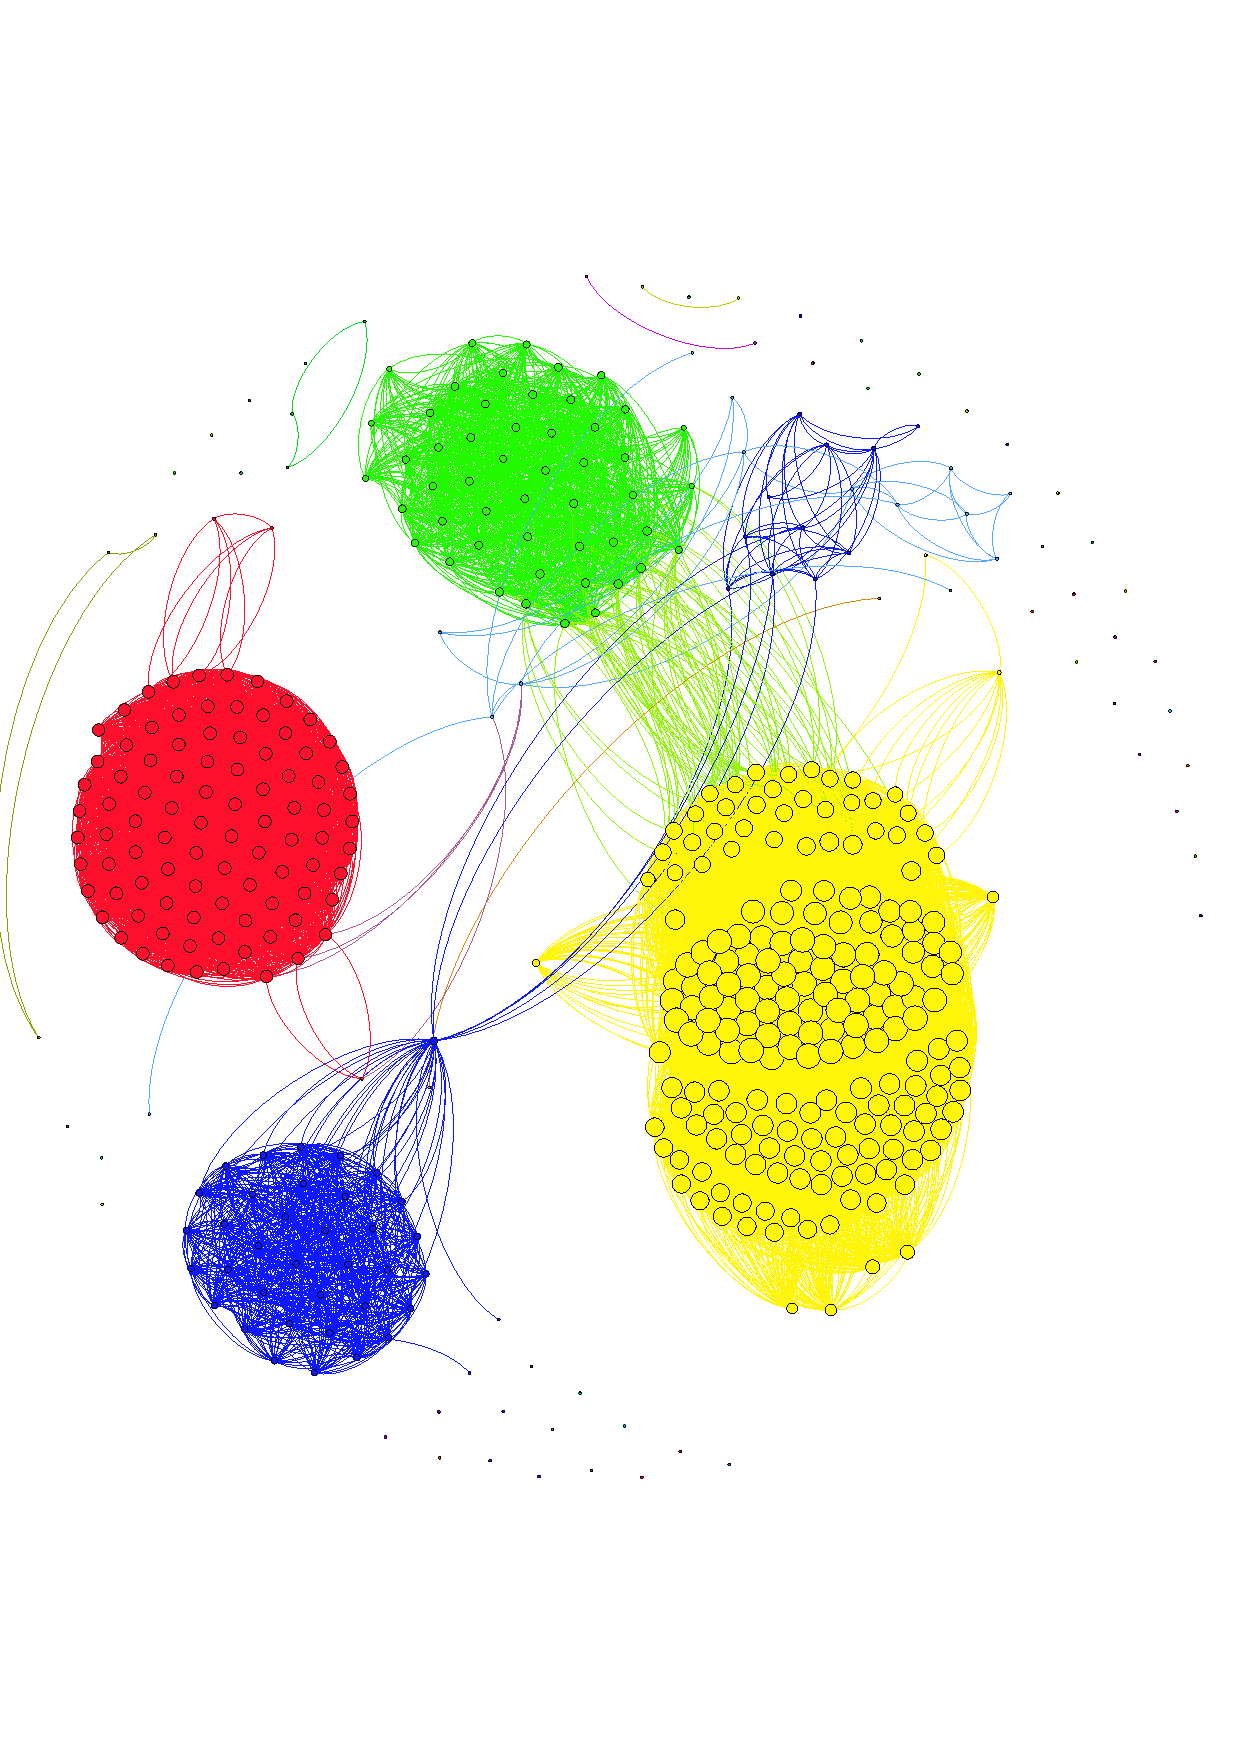
\includegraphics[trim = 0 4cm 2mm 5cm, clip, width=0.45\linewidth]{FileAccess/figs/6261_jacc_pt5}
& 
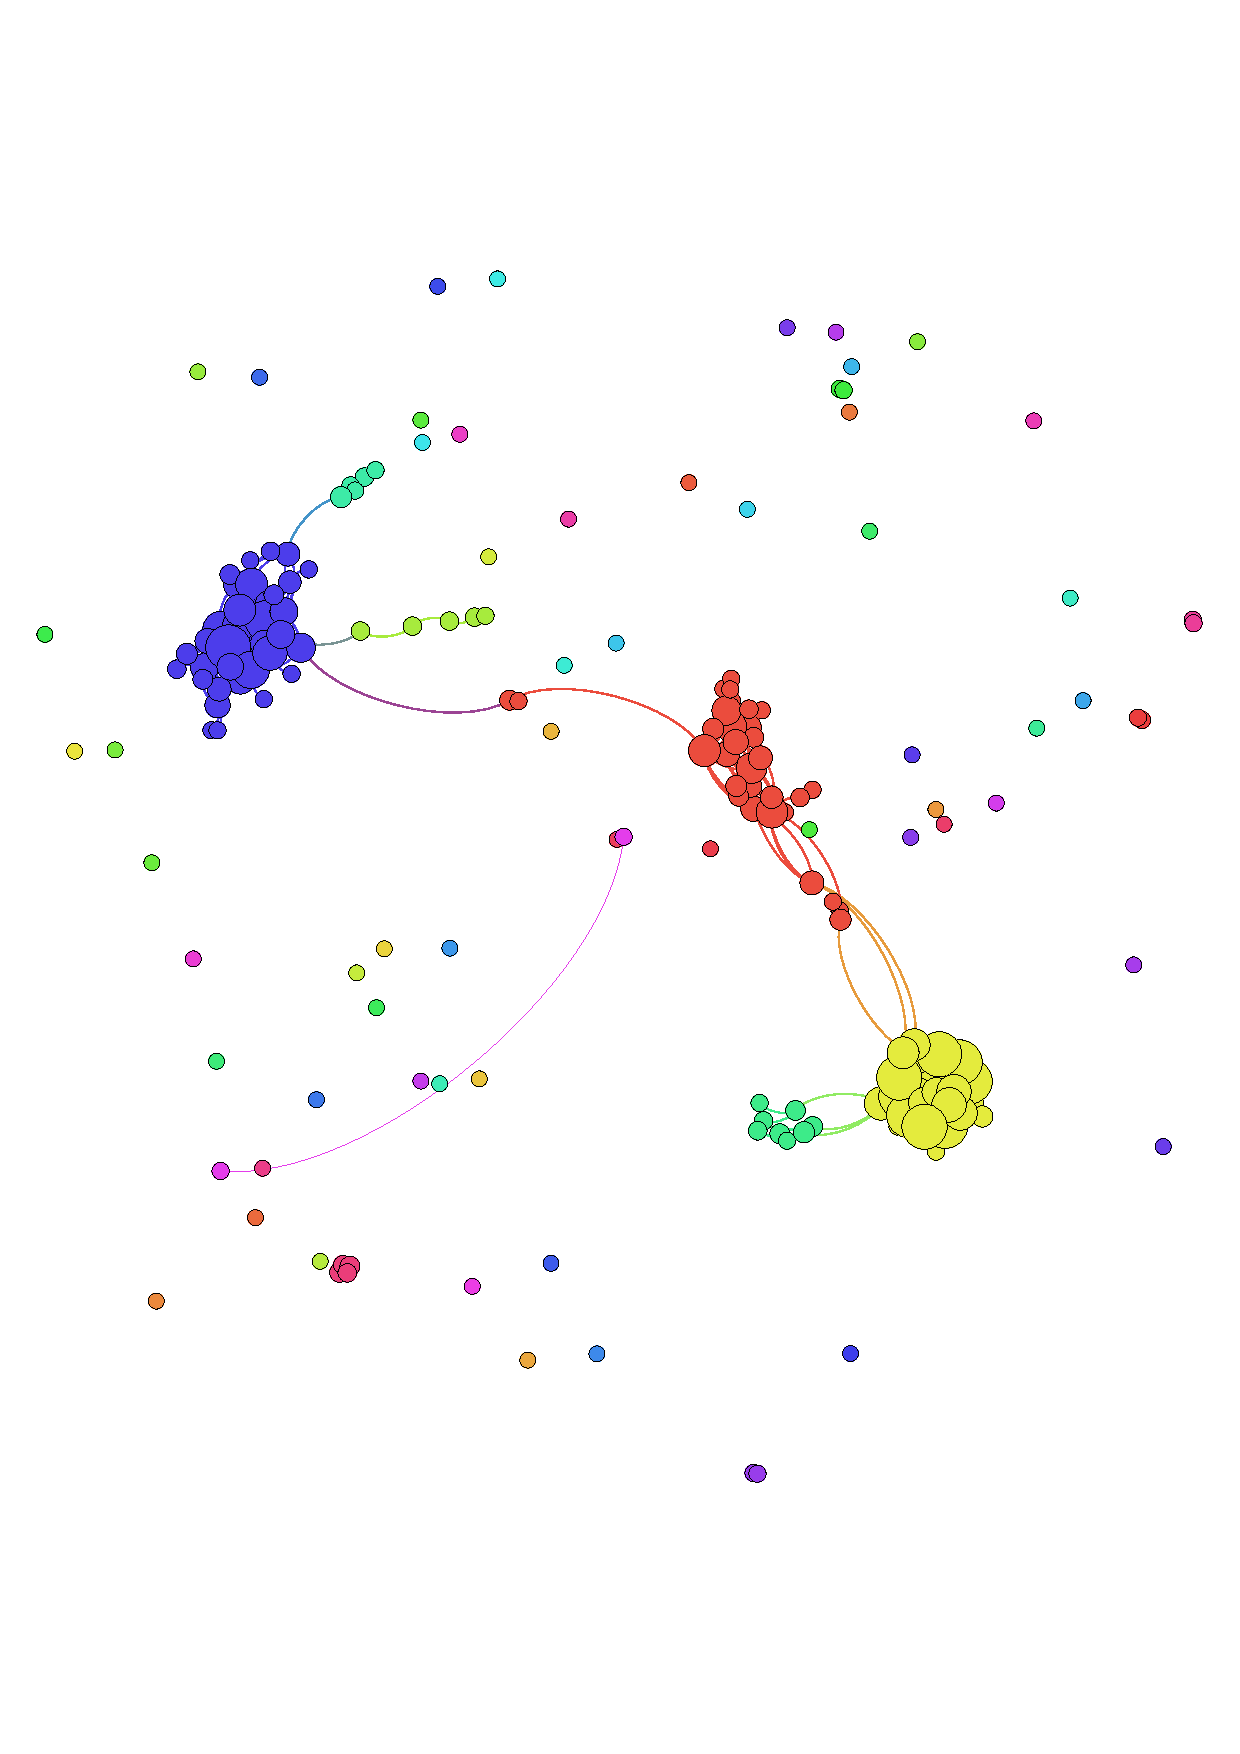
\includegraphics[trim = 2mm 4cm 7mm 5cm, clip, width=0.46\linewidth]{FileAccess/figs/6216_jacc_pt5} \\ 
(a) Share B & (b) Share D \\ 
\end{tabular}
%%
\caption[Social network graphs for shares show that users collaborate
  and tend to form communities by accessing common files. ]{Social network graphs for shares show that users collaborate
  and tend to form communities by accessing common files.  In these
  graphs, each node corresponds to a user, and an edge connects two users
  when the Jaccard index of common files accessed by those users is
  above $0.5$.}
%%
\label{fig:snagraphs}
\end{figure*}
We use file activity logs from eight network file shares of an
enterprise customer for evaluation.  Table~\ref{tab:datasetstats1}
provides key statistics of this data.  Because our recommendation
system targets user collaborations, we select shares from
90\textsuperscript{th} percentile in terms of triangle count -- a
metric to capture degree of collaboration among users.  Triangle count
for a share is the number of triangles formed, where a triangle edge
corresponds to a connection between two users based on accessing at
least one common file.  The table shows the triangle count values
normalized with respect the number of files.  For better
visualization, see Figure~\ref{fig:snagraphs} that shows users forming
different communities based on their collaborations. \\

%% We use the activity log data from eight network file servers (shares) of an enterprise customer for evaluation.
%% %The reader is directed to \cite{dwiticeis15} for details on workload statistics and popular files in these shares. 
%% The selected shares fall in the 90\textsuperscript{th} percentile in
%% terms of total number of triangle counts, i.e., number of triangles
%% formed when two users are connected if there exists at least one file
%% that both users have accessed. Table~\ref{tab:datasetstats1} captures
%% their key statistics. We measure the collaboration among users in a share based on the triangle counts normalized with respect to the number
%% of files. Figures~\ref{fig:snagraphs}(a) and (b) show the social
%% network graphs for users in two shares. It can be seen that the users tend to
%% form communities by co-accessing files.

\noindent\textbf{Removal of automated activity}: 
\label{sec:removebursts}
%%
We observe two types of file activities in our data.  The first
corresponds to the activities that are manually initiated by
users. These activities are characterized by a low number of file
operations per hour.  The second corresponds to scripted activities
that are performed by automated computer programs or scripts.  These
activities are generally seen as bursts or exceptionally high number
of file operations per hour.  Since our goal is to assist knowledge
workers and not automated programs, we need to remove the scripted
activity from the evaluation data.  For this purpose, we remove
the activities by a user in an hours if the number of activities are 
determined to be exceptionally high. Towards this, an appropriate threshold 
is determined using Tukey's outlier
factor~\cite{wang2011statistical}.\linebreak

%% We note from our data that user file activities typically constitute of two modes of operation. The first corresponds to users deliberately performing an action in the file system and is characterized by low number of file operations per hour. The second mode corresponds to scripted activity performed by computer programs or scripts and is seen as bursts or exceptionally high number of file operations per hour. Since our system is designed to assist knowledge workers and not automated computer programs operating from their accounts, the scripted activity should be removed from the evaluation data. We approach this as an anomaly detection problem and argue that if a user is seen to make a high number of file operations per hours, then a large fraction of the actions were scripted. We use Tukey's outlier factor~\cite{wang2011statistical} to determine an appropriate threshold on the number of activities per user per hour. The activity by a user in an hour is labeled scripted and removed if the number of file operations by the user in the hour are above the calculated threshold. 
%% %In order to avoid discarding actual user activity, the threshold is empirically set to 1000 which is above the threshold calculated using~\cite{wang2011statistical}. If a user is seen as making more than 1000 file operations per hour, then a large fractions of the actions were scripted. 
%% The data obtained after removal of scripted activity is used for the rest of the paper. 

\noindent\textbf{Selection of evaluation users}: 
\label{sec:selectusers} 
%
Since our system helps users discover new or modified content, it is
primarily targeted for active users.  Therefore, for each share, we
sample 30 users from the highest quartile of users in terms of number
of activities, and use them in our evaluation.
%% Since our system helps users discover new or modified content, it is most useful for active users. Thus for each evaluation share, we sample 30 users from the highest quartile of users in terms of number of activities, and use them to evaluate our system. 
%
\subsection{Evaluation Methodology}
\label{evalmethodology}
%%
We experiment with different training and testing periods to evaluate the
performance of our system under different settings. 

%%
%Per user models are trained over the training period and tested on actual user activities in the testing period. Experiments are conducted by varying the training and testing periods as described below. 

%% We experiment with different training and testing periods to study the performance of our system under different settings. 
%% %Per user models are trained over the training period and tested on actual user activities in the testing period. Experiments are conducted by varying the training and testing periods as described below. 

\subsubsection{Varying training and test periods} 
\label{sec:varytraintest} 
\begin{figure}[!htbp]
\begin{center}
\centering
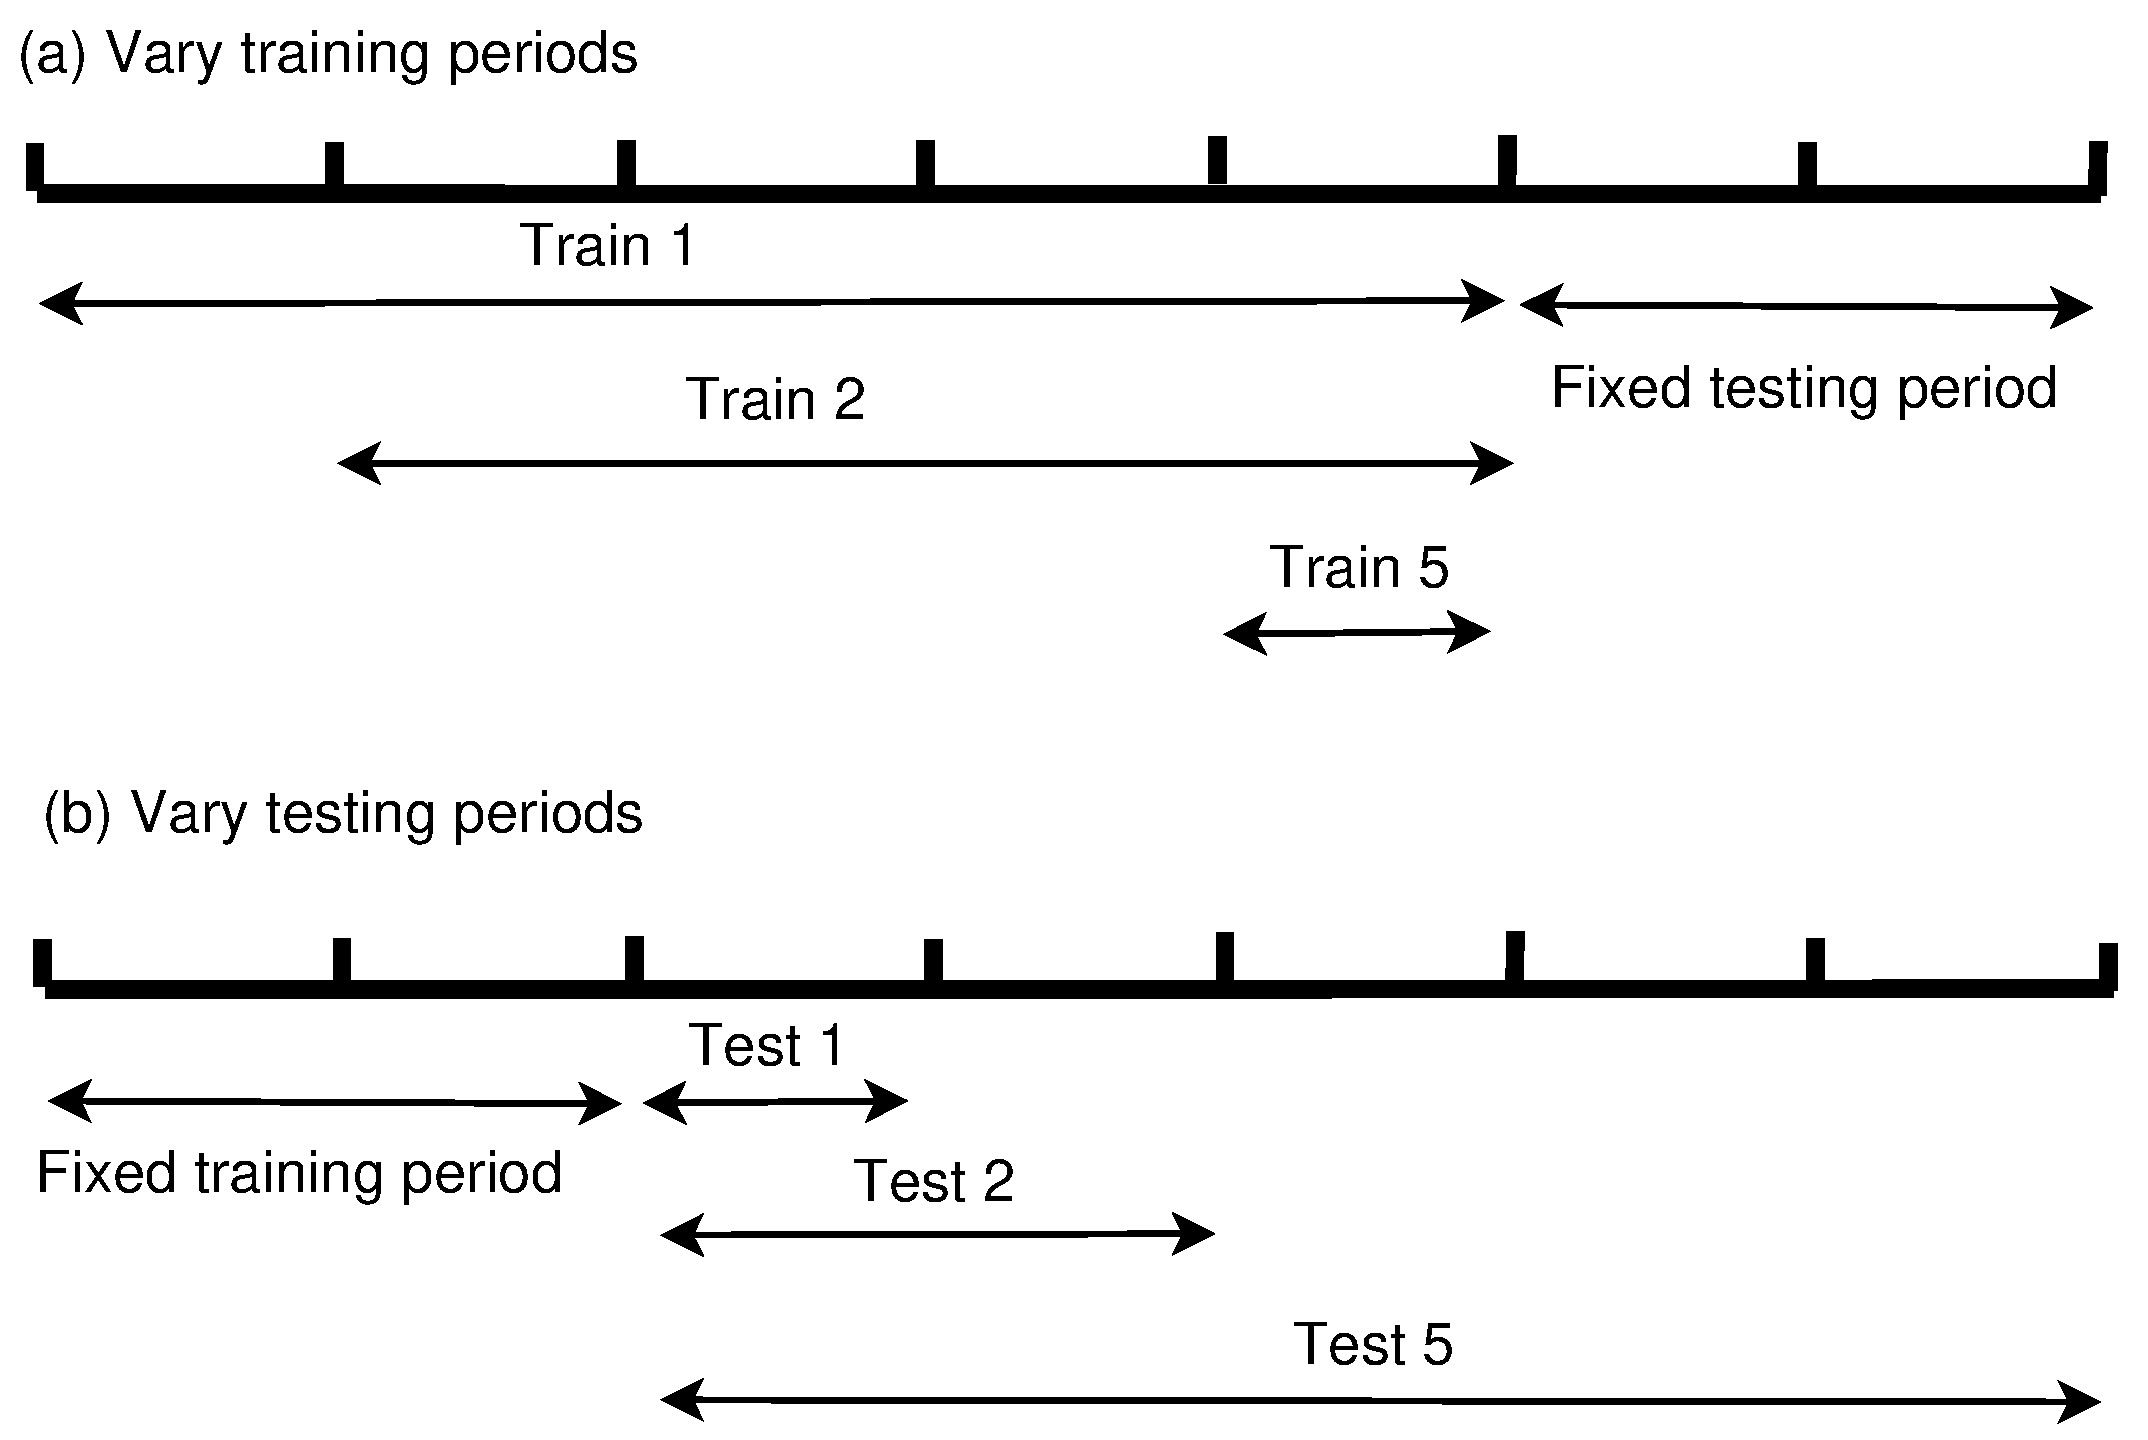
\includegraphics[width=0.75\linewidth]{FileAccess/figs/traintestsplits}
\caption{Splitting dataset into various training and testing periods
%The training period is used for feature extraction and model
%training, and the testing period is used for evaluation of the
%trained models.
} 
\label{fig:traintestsplits}
\end{center}
\end{figure}
%%
We divide the total duration of data from each share into several
slices and create training and testing periods such that testing
occurs immediately after training. For consistency, each share is
divided into seven slices and five training and five testing periods
are created as shown in Figure~\ref{fig:traintestsplits}.
We perform experiments with different combinations:
\begin{itemize}
  \renewcommand{\labelitemi}{$\bullet$}
\item\textbf{Fix testing, vary training.}  A longer training window has
  more number of activities, thereby allowing better model training. 
 However the activities become older as the
  distance between them and the testing period increases, thus preventing the model from reflecting the latest user patterns accurately.  On the
  other hand, a small training window has less number of activities,
  but these activities are relatively fresh.  Thus, there exists a
  trade-off between the size and the \textit{recency} of the training data.
  We study this trade-off by varying the training duration, while
  keeping the testing period fixed.
\item\textbf{Fix training, vary testing.}  As a user's behavior
  evolves over time, it is expected that the effectiveness of the
  user's model would degrade as the testing period becomes longer.  We
  can measure the robustness of a model by observing the rate of
  degradation.  With this goal, we experiment with varying testing
  periods, while keeping the training period fixed.
\end{itemize}
%We next discuss the metrics used to evaluate the performance of our system. 

%% We divide the total duration of data from each share into several slices and create training and testing periods such that testing occurs immediately after training. For consistency, each share is divided into seven slices and five training and five testing periods are created as shown in Figure~\ref{fig:traintestsplits}. 
%% %The total duration of data available from each share is divided into seven slices and several training and testing periods are created (Figure~\ref{fig:traintestsplits}). 
%% The following sets of experiments are conducted. %while ensuring the training and testing periods are adjacent to each other. 

%% \textbf{Fix testing, vary training.}  Given a testing period, a shorter and hence \textit{nearer} training period uses more recent activity however the amount of training data is less. We study this trade-off in model performance by varying the training duration and keeping the testing period fixed. 

%% \textbf{Fix training, vary testing.} Since user behavior may evolve over time, it is expected that the accuracy of trained models would degrade as testing a longer duration. We validate this intuition by fixing the training period and varying testing periods. 

%% %We next discuss the metrics used to evaluate the performance of our system. 

\subsubsection{Evaluation metrics}
\label{sec:metrics}
%%
Consider an experiment with a certain combination of training and
testing periods for a user $u$.  Let $F_{true +, u}$ denote the set of
files that $u$ accessed in the testing period, and $F_{pred +, u}$
denote the set of files predicted by $u$'s model.  Then the precision
and the recall of the model respectively are $\frac{\mid F_{true +, u}
  \cap F_{pred +, u} \mid}{\mid F_{pred +, u}\mid }$, and $\frac{\mid F_{true +,
    u} \cap F_{pred +, u} \mid}{\mid F_{true +, u}\mid}$.  We use the following
metrics to evaluate the effectiveness of the model.
\begin{itemize}
  \renewcommand{\labelitemi}{$\bullet$}
\item \textbf{F-score}: The F-score for a model is the harmonic mean
  of the precision and the recall, and provides a balanced picture of
  the model's effectiveness.
\item \textbf{Recall@75P}: In practice, it is important for a
  recommendation system to have high precision because a large number
  of false positives may discourage a user from using the system
  altogether.  Therefore, we additionally measure the recall values
  when the precision is high -- 75\%.  This is achieved with the help
  of confidence scores associated with the predicted labels.
\end{itemize} 
The measurements for F-score and Recall@75P are averaged across all
the evaluation users to obtain AF and AR@75P respectively. For each
share, we report the average and the maximum values of AF and AR@75P
across the results over all combinations of training and testing
periods.  Please note that the maximum values provide realistic
performance estimate of a properly tuned system.

%% For a certain training period, a testing period and a user $u$, let $F_{true +, u}$ denote the set of files that $u$ read in testing period, and $F_{pred +, u}$ denote the set of files that the model for $u$ predicts would be accessed by $u$. The precision of the predictions made by the model for $u$ is equal to $\frac{\mid F_{true +, u} \cap F_{pred +, u} \mid}{F_{pred +, u}}$ and the recall is equal to $\frac{\mid F_{true +, u} \cap F_{pred +, u}  \mid}{F_{true +, u}}$. We use the following metrics to evaluate the correctness of trained user models in our system. 
%% \begin{itemize}
%% \item \textbf{F-score}: The F-score for user $u$ is the harmonic mean of the precision and recall for the model of $u$ and provides a balanced picture of the prediction correctness. 
%% \item \textbf{Recall@75P}: Practically, it is important for a recommendation system to have high precision since a large number of false positives in the recommendations may discourage the user from using the system altogether. Therefore, with the help of confidence scores associated with each test file, we set the precision to a high value and also evaluate the system based on its recall when precision is 75\%. 


%% \end{itemize} 
%% The F-score and Recall@75P are averaged across the evaluation users to obtain AF and AR@75P respectively. For each share, we report the average as well as the maximum values of AF and AR@75P across all training and testing periods. The maximum values can provide a realistic estimate of the performance expected from a properly tuned system. 

\section{Performance Evaluation} 
\label{sec:results} 
%%
We evaluate our system using the Python-based scikit-learn
library~\cite{scikit-learn}.  We train models on a 32 core, 64GB,
2.6GHz machine, and conduct testing on a separate 8 core, 32GB, 2.7GHz
machine, leveraging multiple cores with multiprocessing.  We use
3-fold cross-validation to learn the regularization parameter $C$ for
the linear SVM models by varying $C$ over {$\{10^{-2}, 10^{-1}, 1,
  10^{1}, 10^{2}, 10^{3}\}$}.

%% The evaluation of our system is conducted using Python-based scikit-learn library~\cite{scikit-learn}. Training of the models is done on a 32 core, 64GB, 2.6GHz machine where the implementation uses multiprocessing to divide computation load across multiple cores. The testing is done on a 8 core, 32GB, 2.7GHz machine. 
%% %\indent Linear Support Vector Machines (SVMs) are chosen to model user access patterns since they offer high model correctness for low training times \cite{dwiticeis15}. In addition, linear SVMs provide feature weights that can determine the significance of individual features, and can be leveraged for techniques such as Active Feature based Model Selection (Section~\ref{sec:testspeedup}) to significantly reduce testing computation of our system. 
%% We use 3-fold cross-validation to learn the regularization parameter $C$ for the linear SVM models by varying $C$ over {$\{10^{-2},
%%   10^{-1}, 1, 10^{1}, 10^{2}, 10^{3}\}$}.  
%\vspace{-0.2in}
%%
\subsection{Metadata Models} 
\begin{table*}[t!]
{\fontsize{8pt}{1em}\selectfont
\begin{center}
\caption{Performance summary for metadata models.  Performance
  numbers are averaged over 5 iterations with random
  initialization of the linear SVM model training. Numbers are listed
  along with the standard deviations. }
%\begin{tabular}{|p{0.6cm}|@{\hspace{0.05in}}p{1.2cm}|@{\hspace{0.03in}}p{1.2cm}|@{\hspace{0.03in}}p{1.2cm}|@{\hspace{0.03in}}p{1.2cm}|>{\raggedleft}p{1.2cm}|}
\begin{tabular}{|c|r|r|r|r|r|}
		\hline
		\textbf{Share} & \textbf{Avg AF} & \textbf{Max AF} & \textbf{Avg AR@75P} & \textbf{Max AR@75P} & \textbf{\% TP by others} \tabularnewline
		\hline
%A&\textbf{37.7}$\pm$0.0&\textbf{40.3}$\pm$0.0&\textbf{0.8}$\pm$0.0&\textbf{1.6}$\pm$0.2&\textbf{84}$\pm$0.0\tabularnewline \hline
A&\textbf{80.7}$\pm$0.0&\textbf{91.1}$\pm$0.0&\textbf{77.6}$\pm$0.0&\textbf{93.9}$\pm$0.0&\textbf{20.4}$\pm$0.0\tabularnewline \hline
B&\textbf{46.4}$\pm$0.0&\textbf{51.2}$\pm$0.0&\textbf{34.9}$\pm$0.0&\textbf{44.2}$\pm$0.0&\textbf{73.1}$\pm$0.0\tabularnewline \hline
C&\textbf{23.1}$\pm$0.0&\textbf{24.2}$\pm$0.0&\textbf{11.4}$\pm$0.0&\textbf{12.4}$\pm$0.0&\textbf{87.7}$\pm$0.0\tabularnewline \hline
D&\textbf{30.7}$\pm$0.0&\textbf{36.3}$\pm$0.0&\textbf{19.0}$\pm$0.0&\textbf{24.7}$\pm$0.0&\textbf{82.8}$\pm$0.0\tabularnewline \hline
E&\textbf{26.9}$\pm$0.0&\textbf{35.0}$\pm$0.0&\textbf{17.9}$\pm$0.0&\textbf{24.1}$\pm$0.0&\textbf{66.0}$\pm$0.0\tabularnewline \hline
F&\textbf{81.5}$\pm$0.0&\textbf{84.3}$\pm$0.0&\textbf{82.9}$\pm$0.0&\textbf{84.6}$\pm$0.0&\textbf{9.8}$\pm$0.0\tabularnewline \hline
G&\textbf{44.8}$\pm$0.0&\textbf{51.3}$\pm$0.0&\textbf{50.6}$\pm$0.0&\textbf{58.3}$\pm$0.0&\textbf{99.9}$\pm$0.0\tabularnewline \hline
H&\textbf{47.6}$\pm$0.0&\textbf{50.2}$\pm$0.0&\textbf{49.9}$\pm$0.0&\textbf{53.0}$\pm$0.0&\textbf{74.4}$\pm$0.0\tabularnewline \hline
%J&\textbf{26.6}$\pm$0.0&\textbf{27.2}$\pm$0.0&\textbf{4.7}$\pm$0.0&\textbf{5.8}$\pm$0.0&\textbf{79}$\pm$0.0\tabularnewline \hline
\end{tabular}
\end{center}
%\vspace{-0.35in}
\label{tab:WithoutBurstsPerf} % Note: these are latest. -2/26/15
}
\end{table*}
\begin{table*}[t!]
{\fontsize{8pt}{1em}\selectfont
\begin{center}
\caption{Performance summary for CF models. Performance
  numbers are averaged over 5 iterations with random
  initialization of the linear SVM model training. Numbers are listed
  along with the standard deviations.}
%\begin{tabular}{|p{0.6cm}|@{\hspace{0.05in}}p{1.2cm}|@{\hspace{0.03in}}p{1.2cm}|@{\hspace{0.03in}}p{1.2cm}|@{\hspace{0.03in}}p{1.2cm}|>{\raggedleft}p{1.2cm}|}
\begin{tabular}{|c|r|r|r|r|r|}
		\hline
		\textbf{Share} & \textbf{Avg AF} & \textbf{Max AF} & \textbf{Avg AR@75P} & \textbf{Max AR@75P} & \textbf{\% TP by others} \tabularnewline
		\hline
%A&\textbf{37.4}$\pm$0.1&\textbf{46.1}$\pm$0.0&\textbf{0.5}$\pm$0.0&\textbf{2.6}$\pm$0.0&\textbf{82}$\pm$0.0\tabularnewline \hline
A&\textbf{80.7}$\pm$0.0&\textbf{100.0}$\pm$0.0&\textbf{78.5}$\pm$0.0&\textbf{100.0}$\pm$0.0&\textbf{21.2}$\pm$0.0\tabularnewline \hline
B&\textbf{48.6}$\pm$0.0&\textbf{77.1}$\pm$0.0&\textbf{32.2}$\pm$0.6&\textbf{62.1}$\pm$0.0&\textbf{73.1}$\pm$0.0\tabularnewline \hline
C&\textbf{23.5}$\pm$0.0&\textbf{36.0}$\pm$0.0&\textbf{10.1}$\pm$0.0&\textbf{16.0}$\pm$0.0&\textbf{87.5}$\pm$0.0\tabularnewline \hline
D&\textbf{32.3}$\pm$0.0&\textbf{47.5}$\pm$0.0&\textbf{21.5}$\pm$0.0&\textbf{38.3}$\pm$0.0&\textbf{83.3}$\pm$0.0\tabularnewline \hline
E&\textbf{27.6}$\pm$0.0&\textbf{41.1}$\pm$0.0&\textbf{25.3}$\pm$0.0&\textbf{100.0}$\pm$0.0&\textbf{65.7}$\pm$0.0\tabularnewline \hline
F&\textbf{81.5}$\pm$0.0&\textbf{87.9}$\pm$0.0&\textbf{83.3}$\pm$0.0&\textbf{89.2}$\pm$0.0&\textbf{9.8}$\pm$0.0\tabularnewline \hline
G&\textbf{55.5}$\pm$0.1&\textbf{76.2}$\pm$0.0&\textbf{58.0}$\pm$0.2&\textbf{89.9}$\pm$0.4&\textbf{96.6}$\pm$0.1\tabularnewline \hline
H&\textbf{47.6}$\pm$0.0&\textbf{57.2}$\pm$0.0&\textbf{49.6}$\pm$0.0&\textbf{66.5}$\pm$0.0&\textbf{75.4}$\pm$0.0\tabularnewline \hline
%J&\textbf{26.7}$\pm$0.0&\textbf{28.7}$\pm$0.0&\textbf{2.9}$\pm$0.0&\textbf{5.6}$\pm$0.0&\textbf{79}$\pm$0.0\tabularnewline \hline
\end{tabular}
\end{center}
}
%\vspace{-0.1in}

\label{tab:CollabFilteringPerf}  % Note: these are latest. -2/26/15 
\end{table*}

Table~\ref{tab:WithoutBurstsPerf} shows performance results of the
metadata models.  The numbers in column Max AR@75P are reasonable
performance estimate of a well tuned system.  The average of these
numbers across all the shares, 49.4\%, shows that our metadata models 
can capture nearly half of users' access for new files, while having under 25\% 
wrong file recommendations. This demonstrates the effectiveness of the 
trained models. 

We would like to point out that our dataset includes an undesirable
case where during the testing phase, a user accesses a new file that 
was recently created by the same user. Since recommending such a file to the
user is not useful, we measure their proportion in our recommendations. 
The last column of Table~\ref{tab:WithoutBurstsPerf} shows that 
most of the correctly recommended files do not fall in the above category, 
thereby upholding the validity of our models.

%% Table~\ref{tab:WithoutBurstsPerf} shows that the performance of the metadata models varies significantly with the evaluation shares. Intuitively, it may not be useful to recommend a file to a user if the file had been recently created by the same user. The last column of Table~\ref{tab:WithoutBurstsPerf} shows that most of the files that are correctly recommended to users do not fall in this category. 

\subsection{CF Models} 
%%
We experimented with different strategies to sample validation files
for training CF models.  We use the strategy that provides the best
performance, which is using the training set itself as the validation
set.  The results in Table~\ref{tab:CollabFilteringPerf} clearly
highlight the significant gains of CF models over metadata models.
The average of Max AR@75P across all shares is 70.2\%, which is an
improvement of a whopping 20\% over the performance of metadata models.
Also, it is not very surprising that the top four shares, B, D, E, and
G, in terms of gains of the CF model, are found in the top five shares in
terms of normalized triangle counts.  Share A, which is the remaining
share in the top five, doesn't show substantial improvement primarily
because the performance of its metadata model is already too high.
%\vspace{-0.2in} 

%% We experimented with different strategies to sample validation files to train CF models. The best performance is observed when the set of validation files is the same as that of the training files. We have used this setting in our experiments. Table~\ref{tab:CollabFilteringPerf} shows that the CF models clearly outperform the metadata models. It can also be seen that most improvement after CF models is seen in shares B, D, E, and G which occur in the top five shares in Table~\ref{tab:datasetstats1} in terms of user collaboration as measured by normalized triangle counts. Although share A is among the top shares in terms of user collaboration, the performance of metadata models on share A is already high and so the improvement by CF models could not be substantial. 
%% %\vspace{-0.2in} 
\subsection{Temporal Variation in Performance}
%\vspace{-0.8cm}
\begin{figure*}
\centering
\begin{minipage}{.95\textwidth}
  \centering
  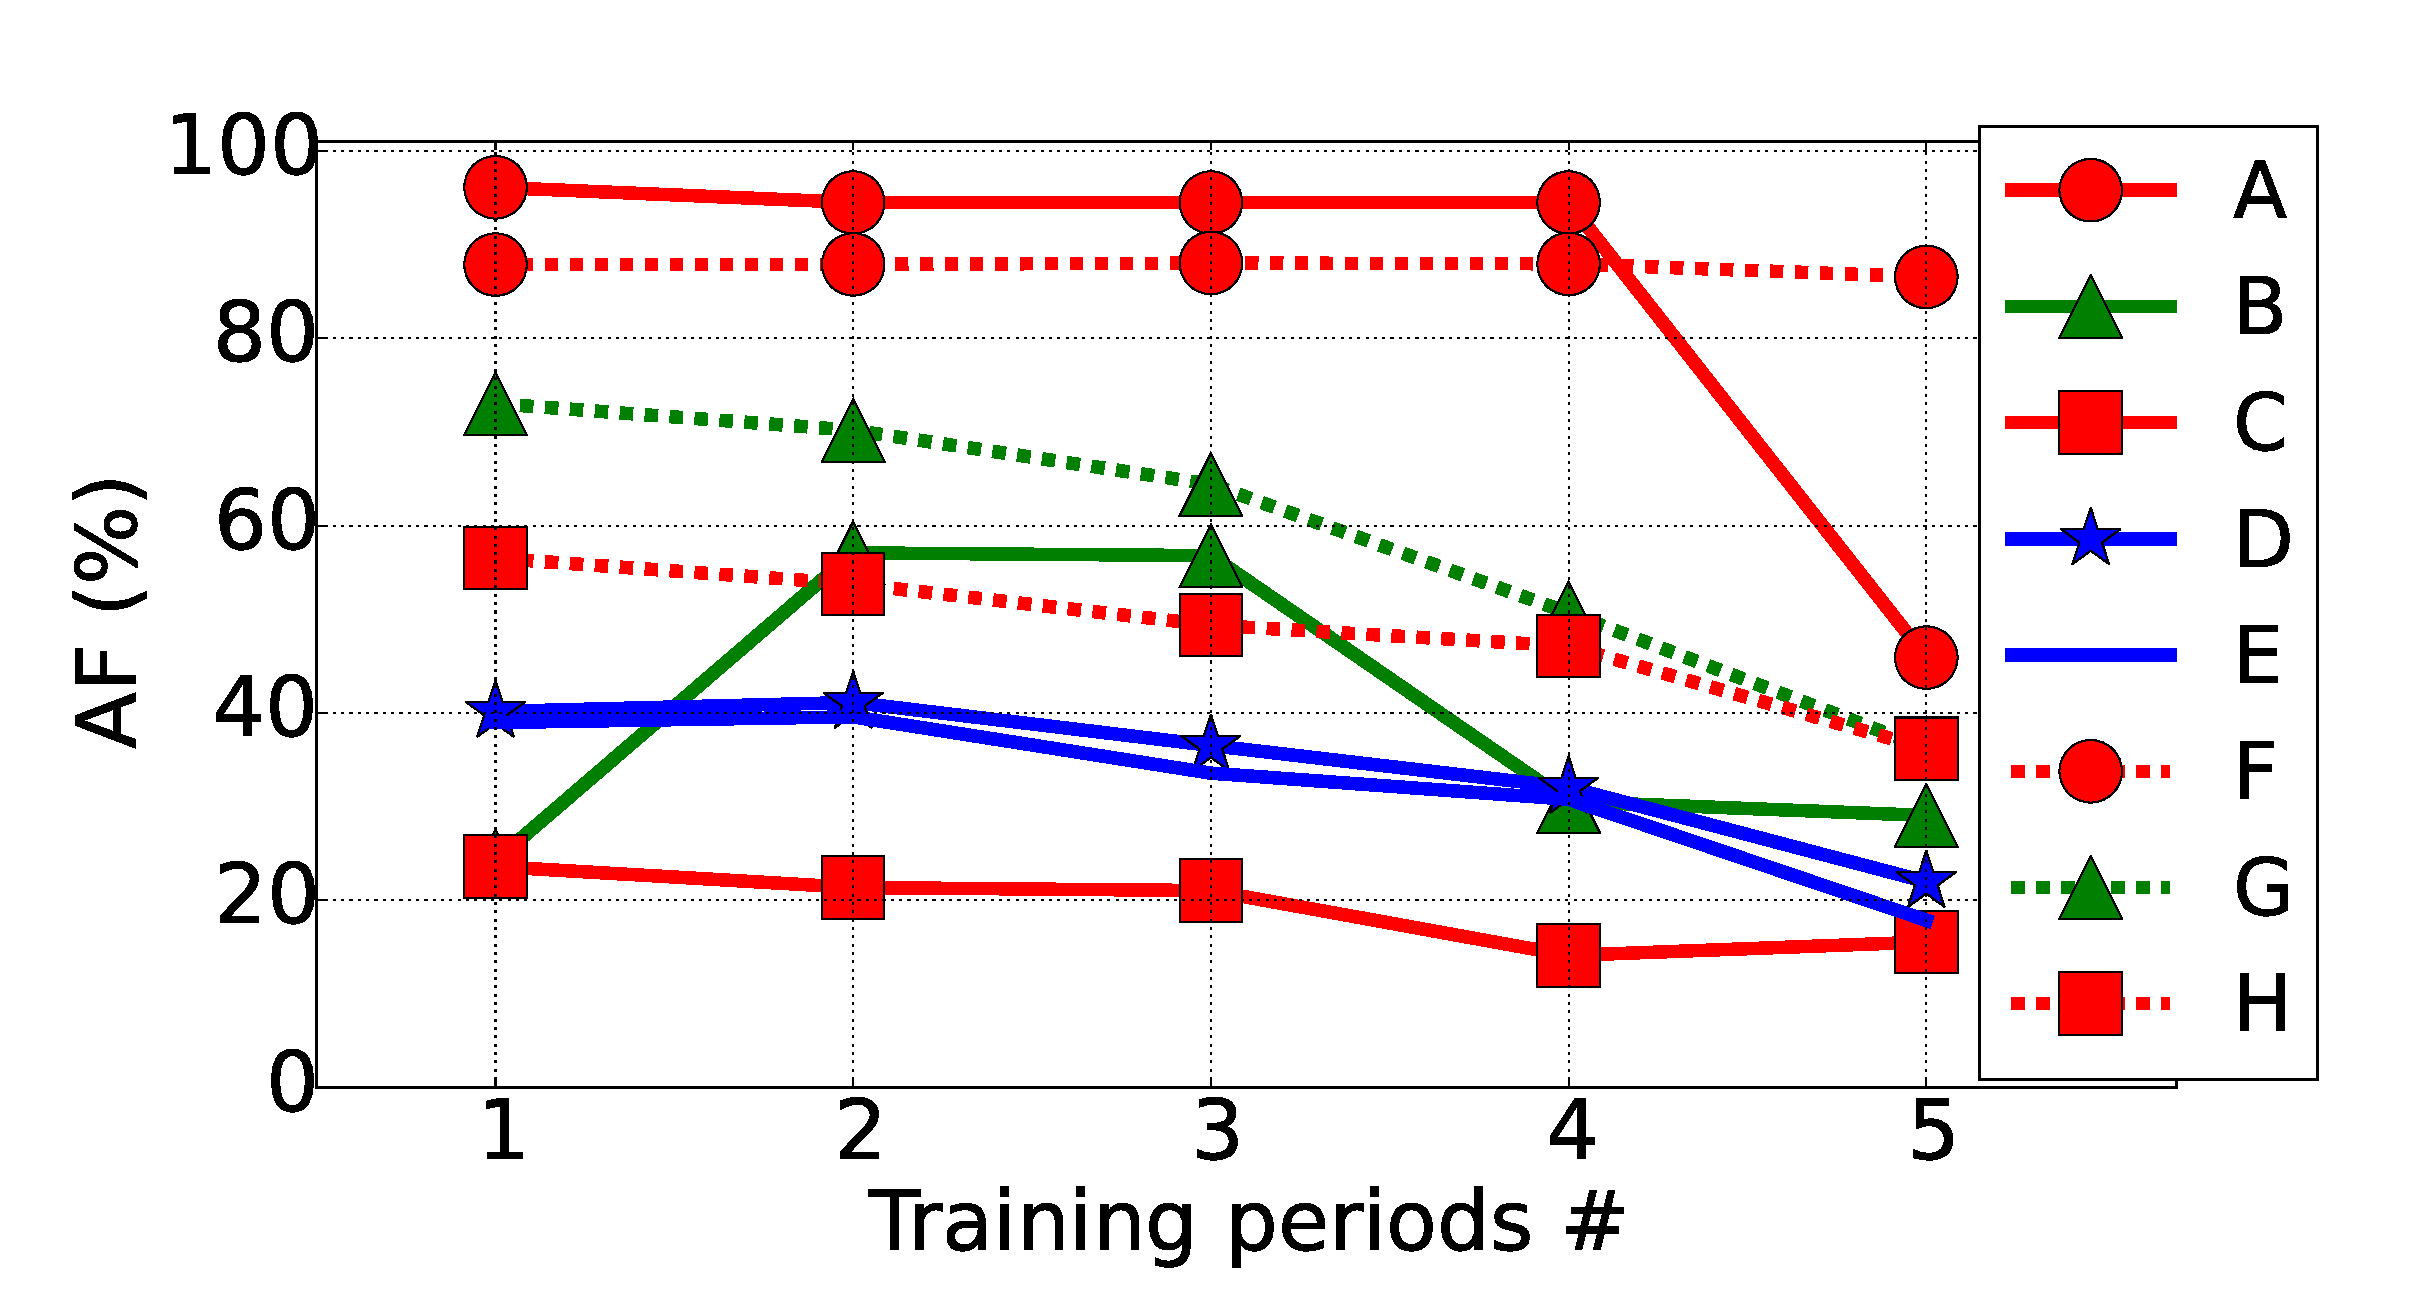
\includegraphics[width=0.65\linewidth]{FileAccess/figs/VaryTrainFScore10}
  \captionof{figure}{AF for metadata models with the fixed testing and varying training periods} 
  \label{fig:varytrainFscore}
%\vspace{-0.5cm}
\end{minipage} % 
\begin{minipage}{.95\textwidth}
  \centering
  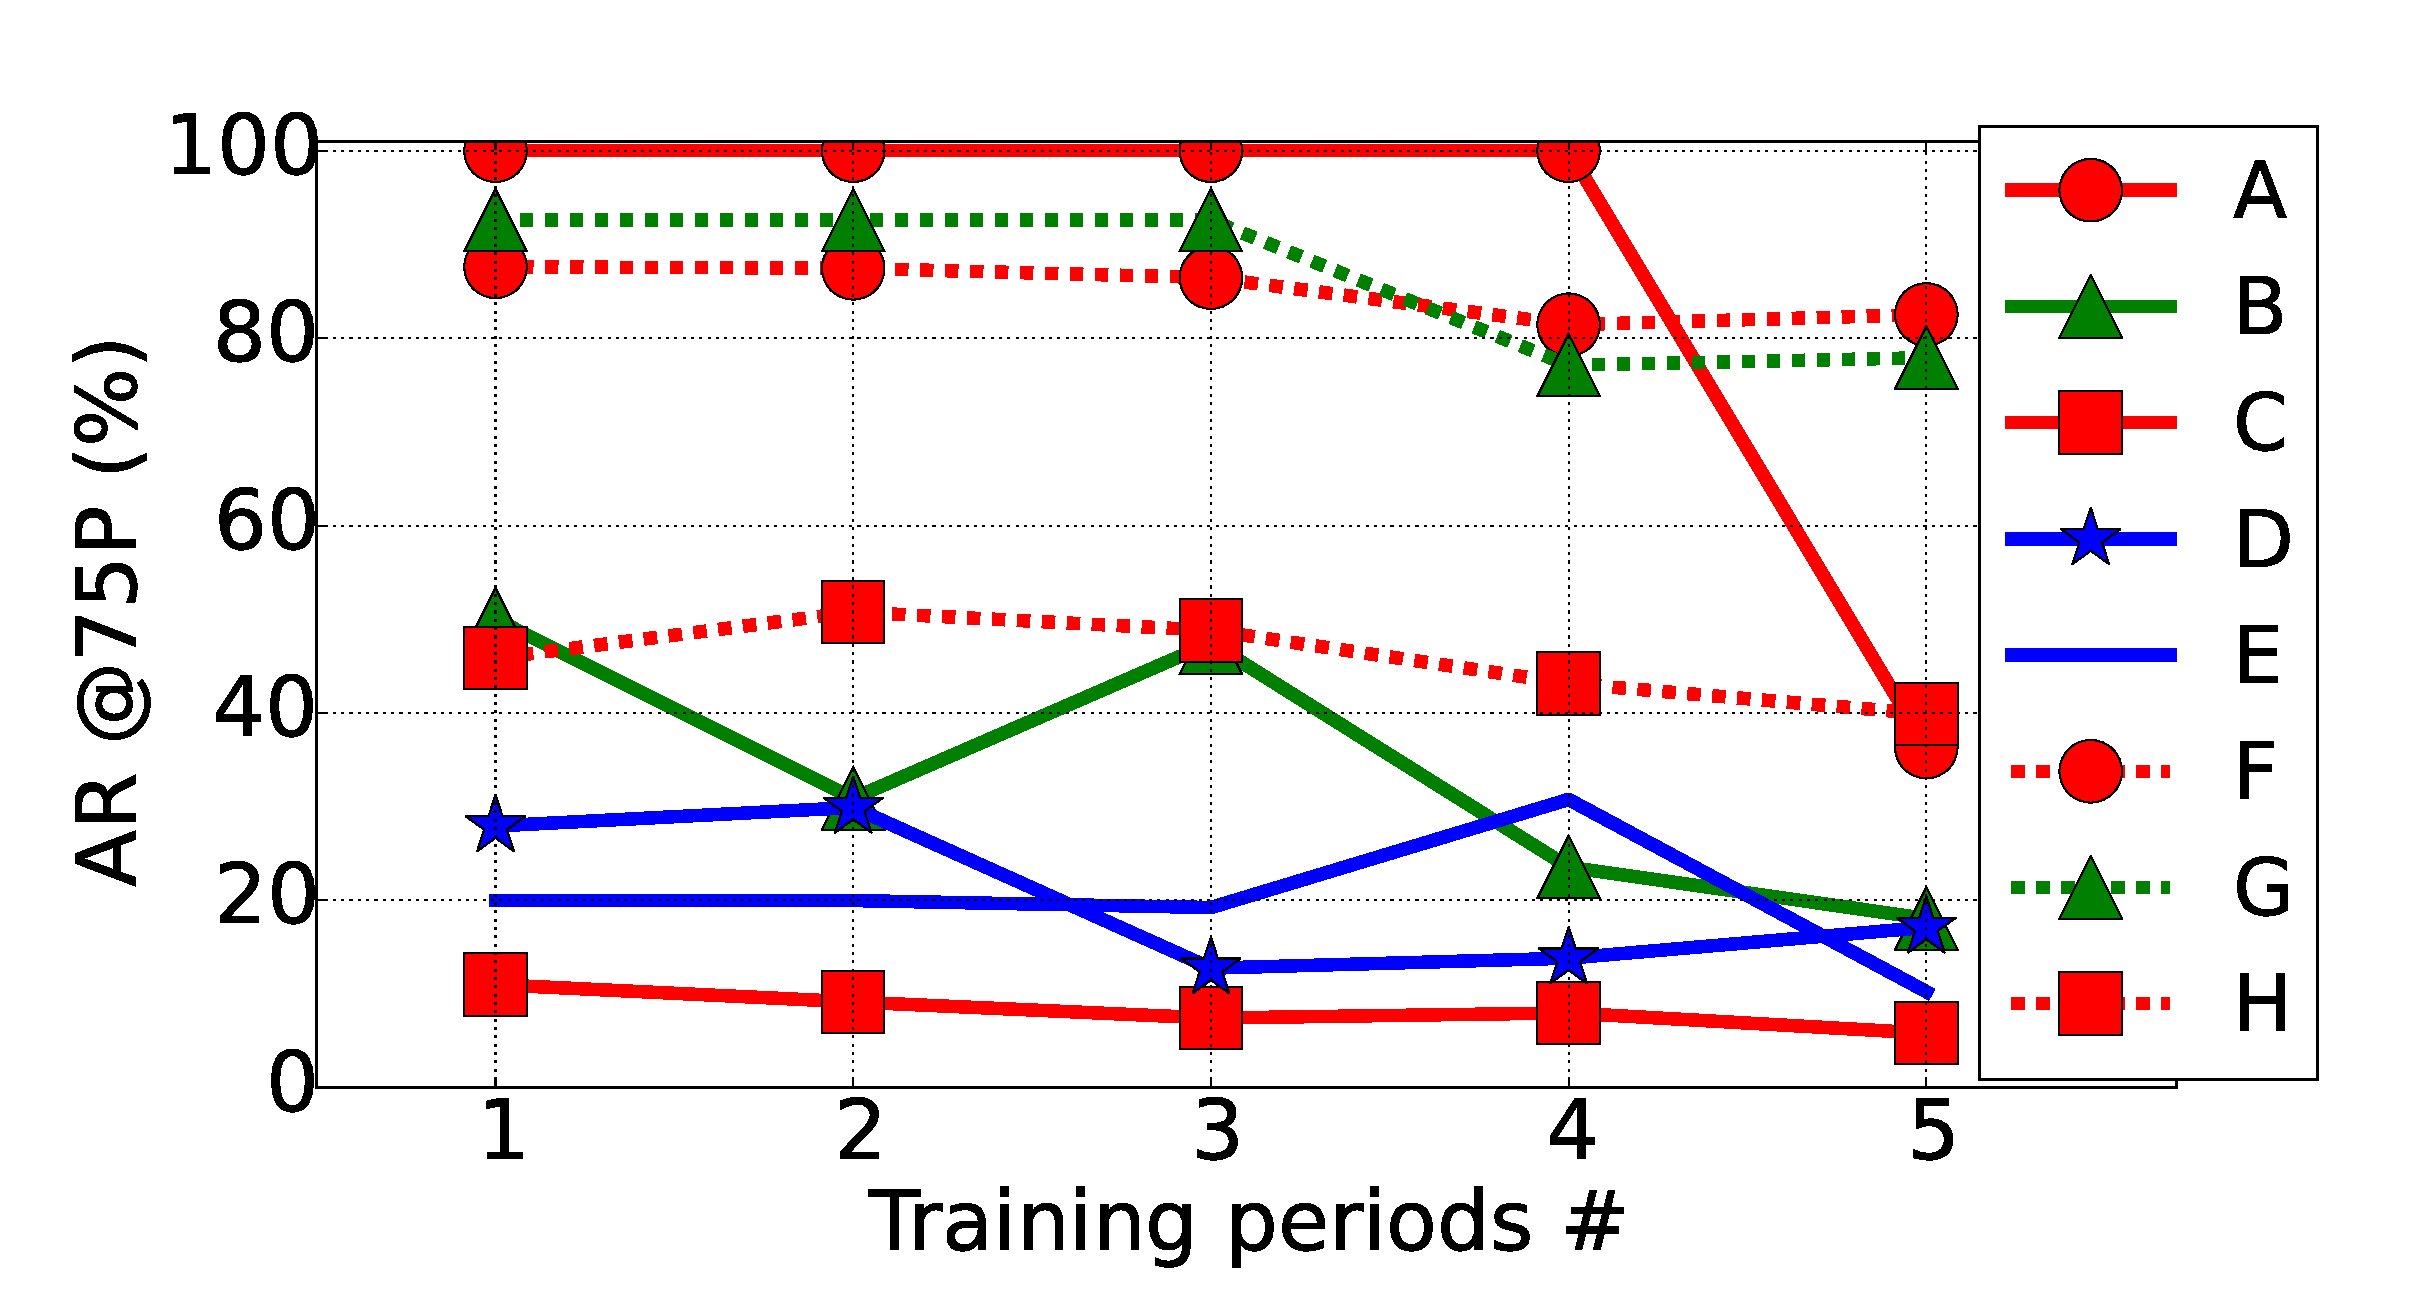
\includegraphics[width=0.65\linewidth]{FileAccess/figs/VaryTrainR7510}
  \captionof{figure}{AR@75P for metadata models with the fixed
    testing and varying training periods}
  \label{fig:varytrainR75}
%\vspace{-0.5cm}
\end{minipage}
\end{figure*}
%\vspace{-0.6cm}

\begin{figure*}
\centering
\begin{minipage}{.95\textwidth}
  \centering
  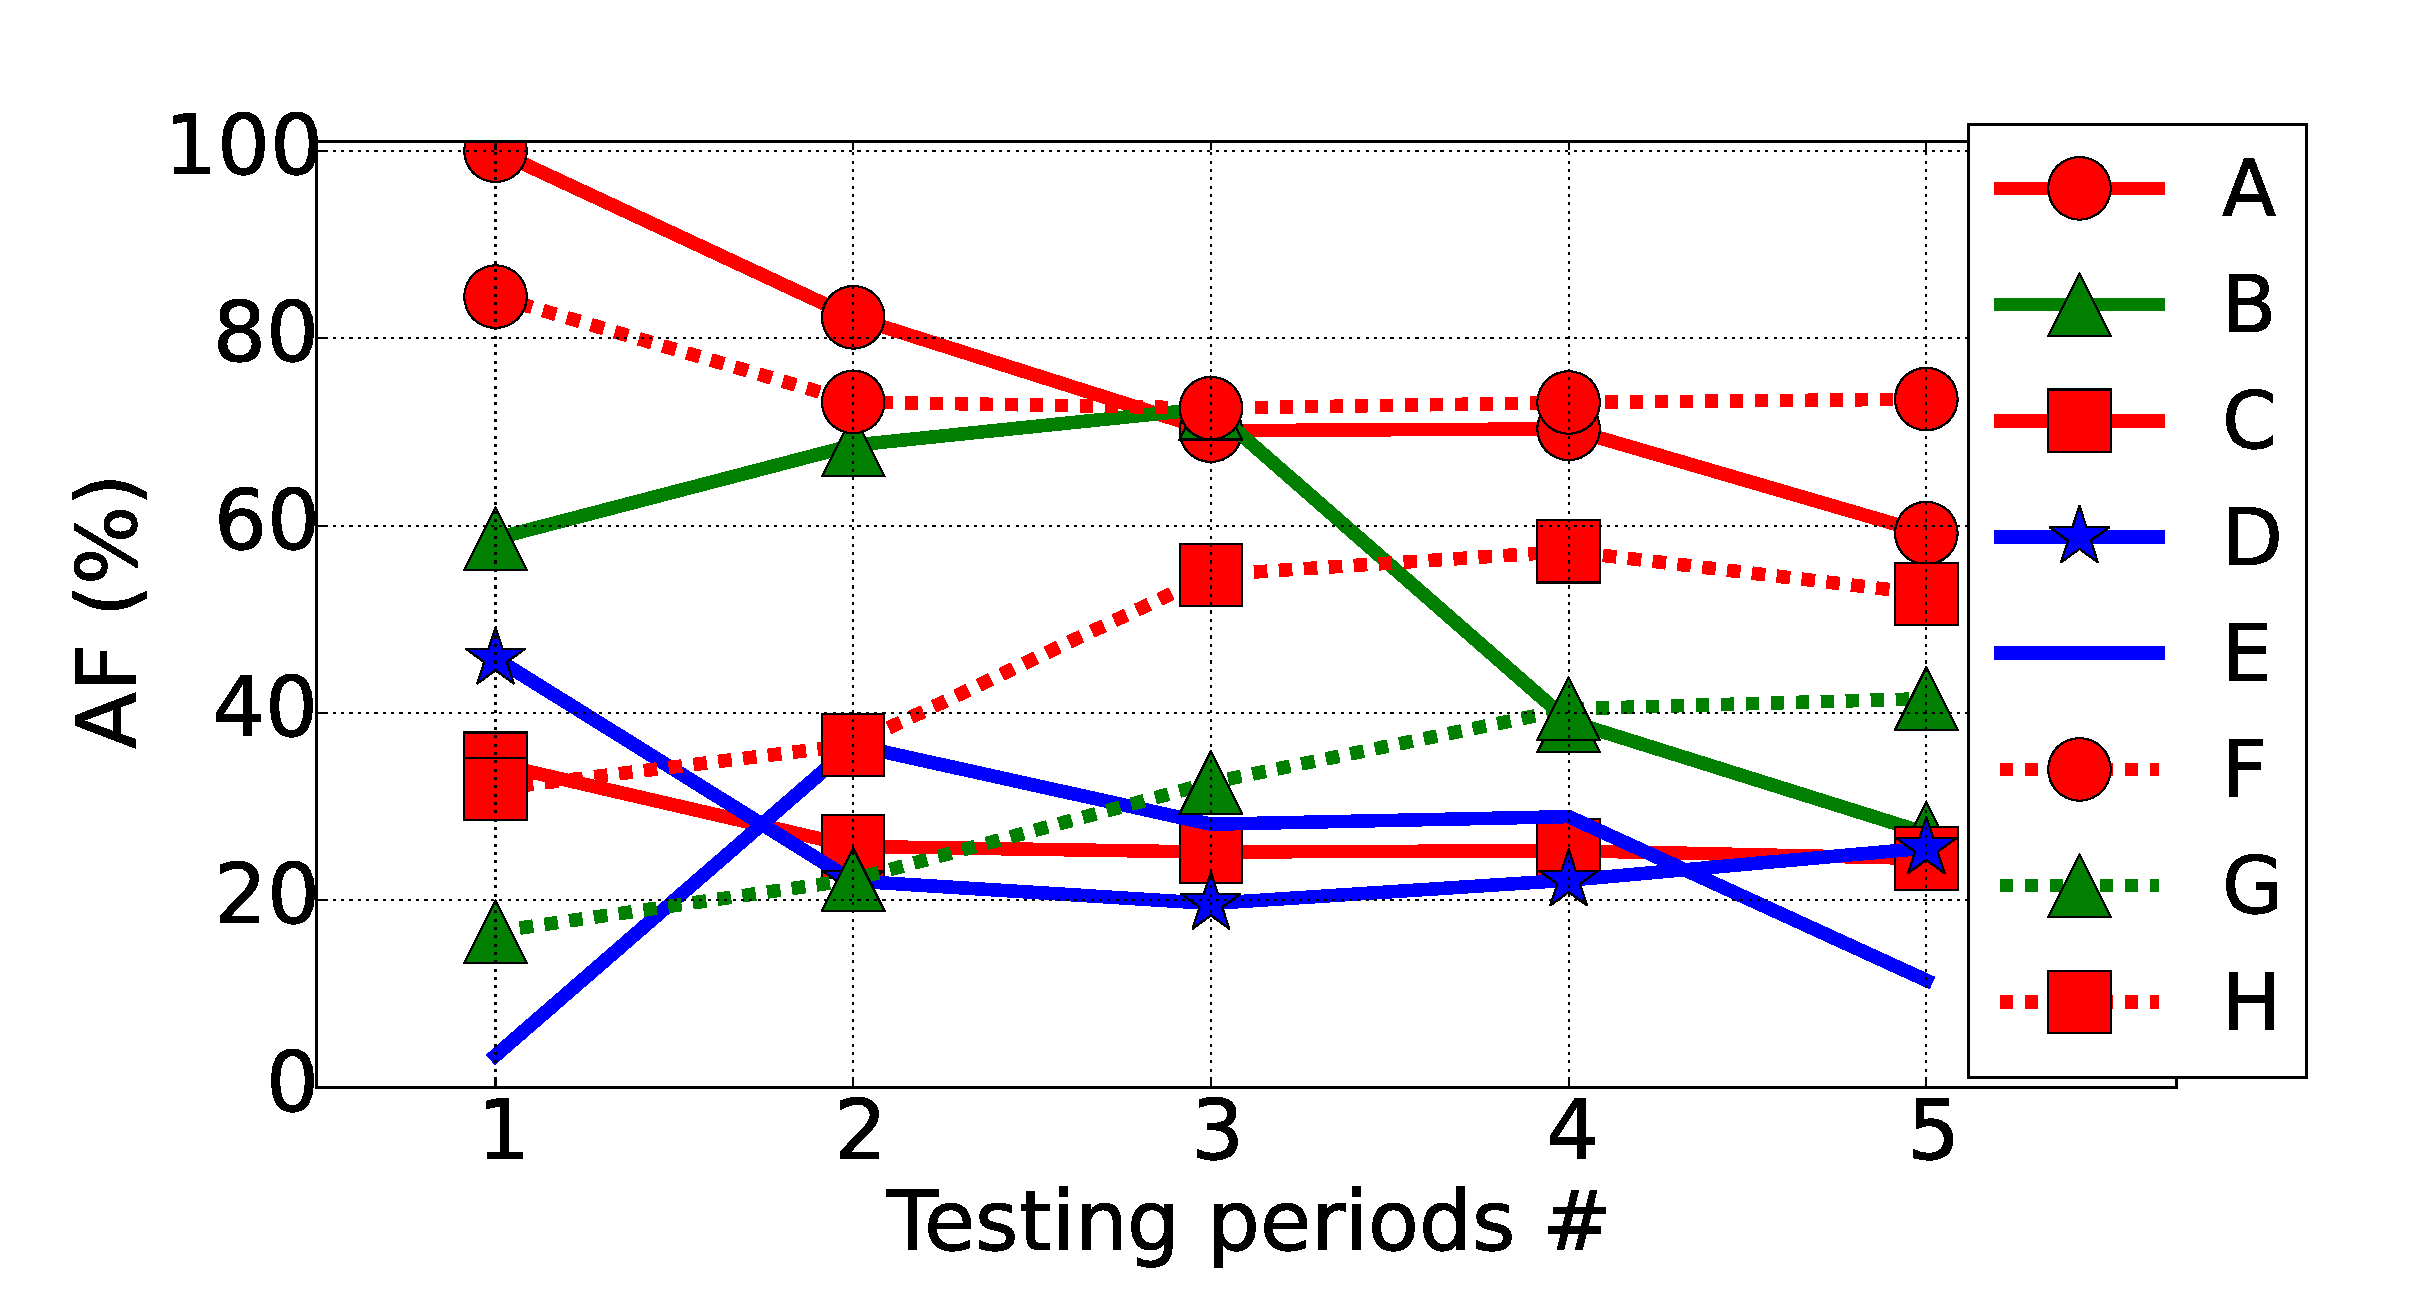
\includegraphics[width=0.65\linewidth]{FileAccess/figs/VaryTestFScore10}
  \captionof{figure}{AF for metadata models with the fixed 
    training and varying test periods}
  \label{fig:varytestFscore}
%\vspace{-0.2cm}
\end{minipage} %
\begin{minipage}{.95\textwidth}
  \centering
  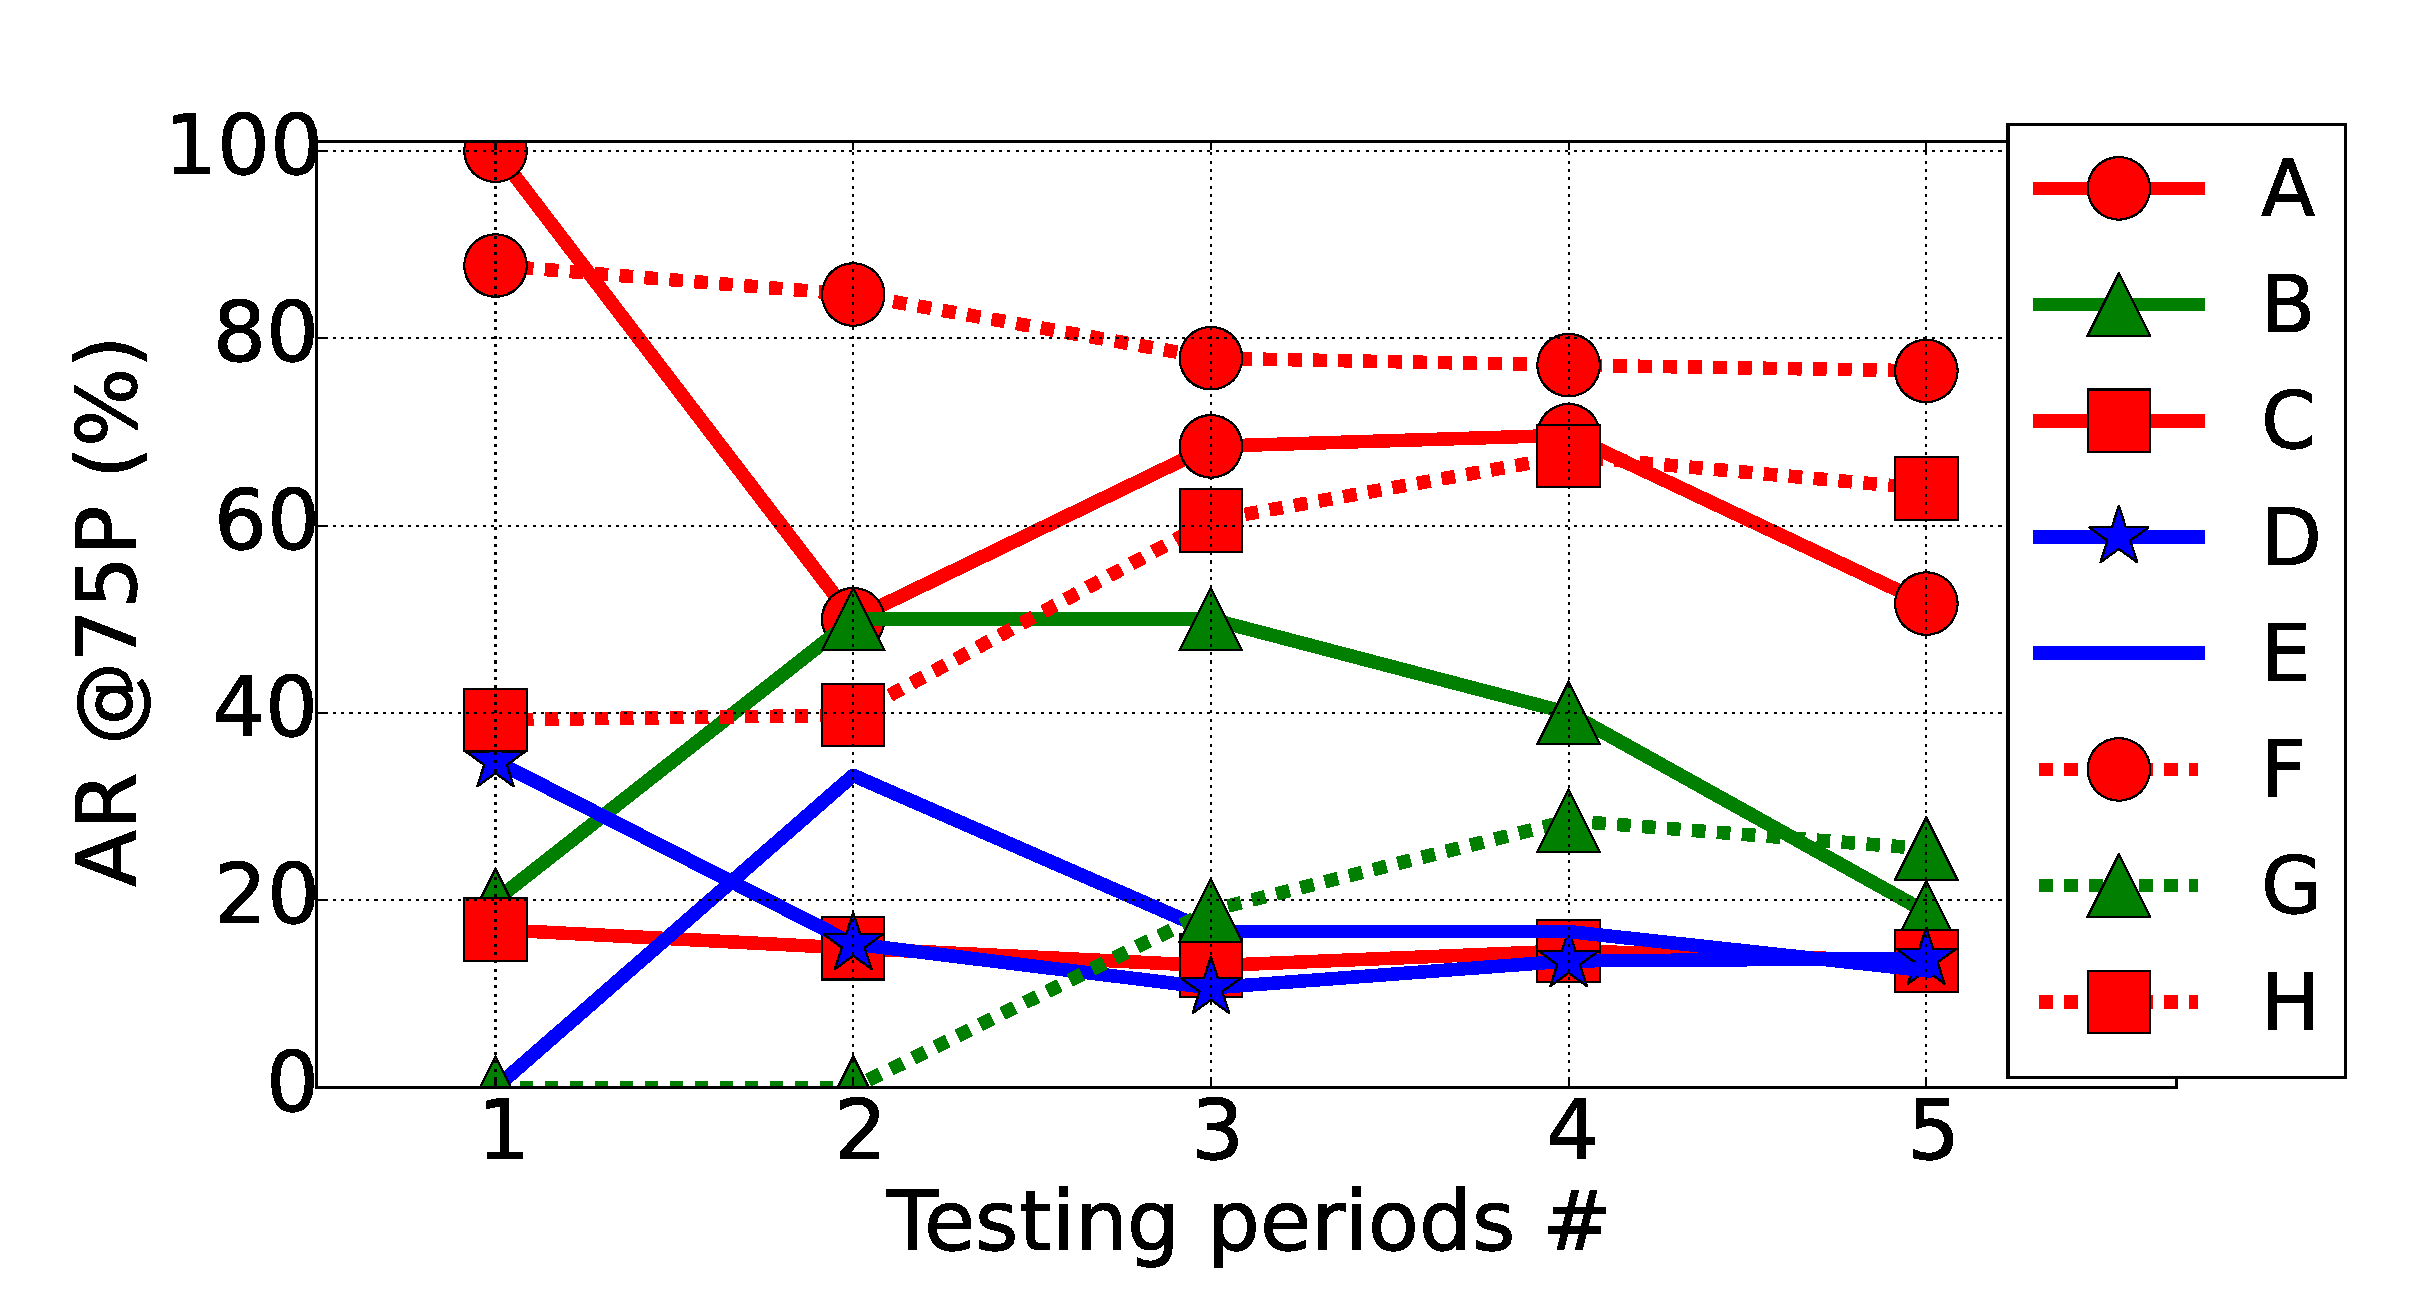
\includegraphics[width=0.65\linewidth]{FileAccess/figs/VaryTestR7510}
  \captionof{figure}{AR@75P for metadata models with the fixed
    training and varying test periods}
  \label{fig:varytestR75}
%\vspace{-0.2cm}
\end{minipage}
%\vspace{-0.1in}
\end{figure*}
%%
%%
To study the performance variations for different lengths of training
and testing periods, we focus only on the metadata models because as
compared to CF models, they provide larger variation owing to lower
baseline performance.


\subsubsection{Varying training period}
%%
Figures~\ref{fig:varytrainFscore} and \ref{fig:varytrainR75} show the
performance variation of metadata models with varying training
periods.  The best performance for most shares is observed for index
$1$ that corresponds to the longest training period.  As expected, the
performance degrades as the training window shrinks.  Performance can
also degrade for a large training window wherein a model gives
importance to activities that are outdated with respect to the user's
recent access pattern.  However, we don't observe this behavior
because the longest training periods, ranging from 41 to 88 days for
the eight shares, are not long enough to cause the degradation.

\subsubsection{Varying testing period}
%%
Figures~\ref{fig:varytestFscore} and \ref{fig:varytestR75} show the
performance variation of metadata models with varying testing periods.
Beyond the testing periods with indices 1 and 2 which are the smallest
and hence potentially the noisiest, the performance degrades mildly as
the testing window widens.  This is an excellent indicator of the
robustness of our models.

%% This section analyzes the performance variation of our system for different training and testing periods, and for different users. Figures~\ref{fig:varytrainFscore} and \ref{fig:varytrainR75} show the performance variation with metadata models when the training period is varied. The best performance for most shares is observed for index $1$ which corresponds to the longest training period. The models experience a moderate degradation in performance for shorter training periods due to reduction in the training data. For extremely large training periods, it is expected that the model performance would degrade since the models would give importance to activity that may be outdated with respect to the user's current access patterns. However the duration of the longest training period in our experiments only varies from 41 to 88 days for the eight shares and such a drop in the performance is not observed. We revisit this point in the context of per-user performance analysis later in this section. Since one training duration may not be optimal for all shares and enterprise environments, we also provide a technique that can enable the tuning of system parameters based on its online evaluation. 

%% Tables~\ref{fig:varytestFscore} and \ref{fig:varytestR75} show how the performance varies for metadata models as the testing periods are varied. Beyond the testing periods with indices 1 and 2 which are the smallest and hence potentially noisiest, a mild drop in performance can be observed as the trained models are used over a longer testing period, indicating longevity of our models. 
%\vspace{-0.3cm}
\begin{figure}[!htbp]
\begin{center}
\centering
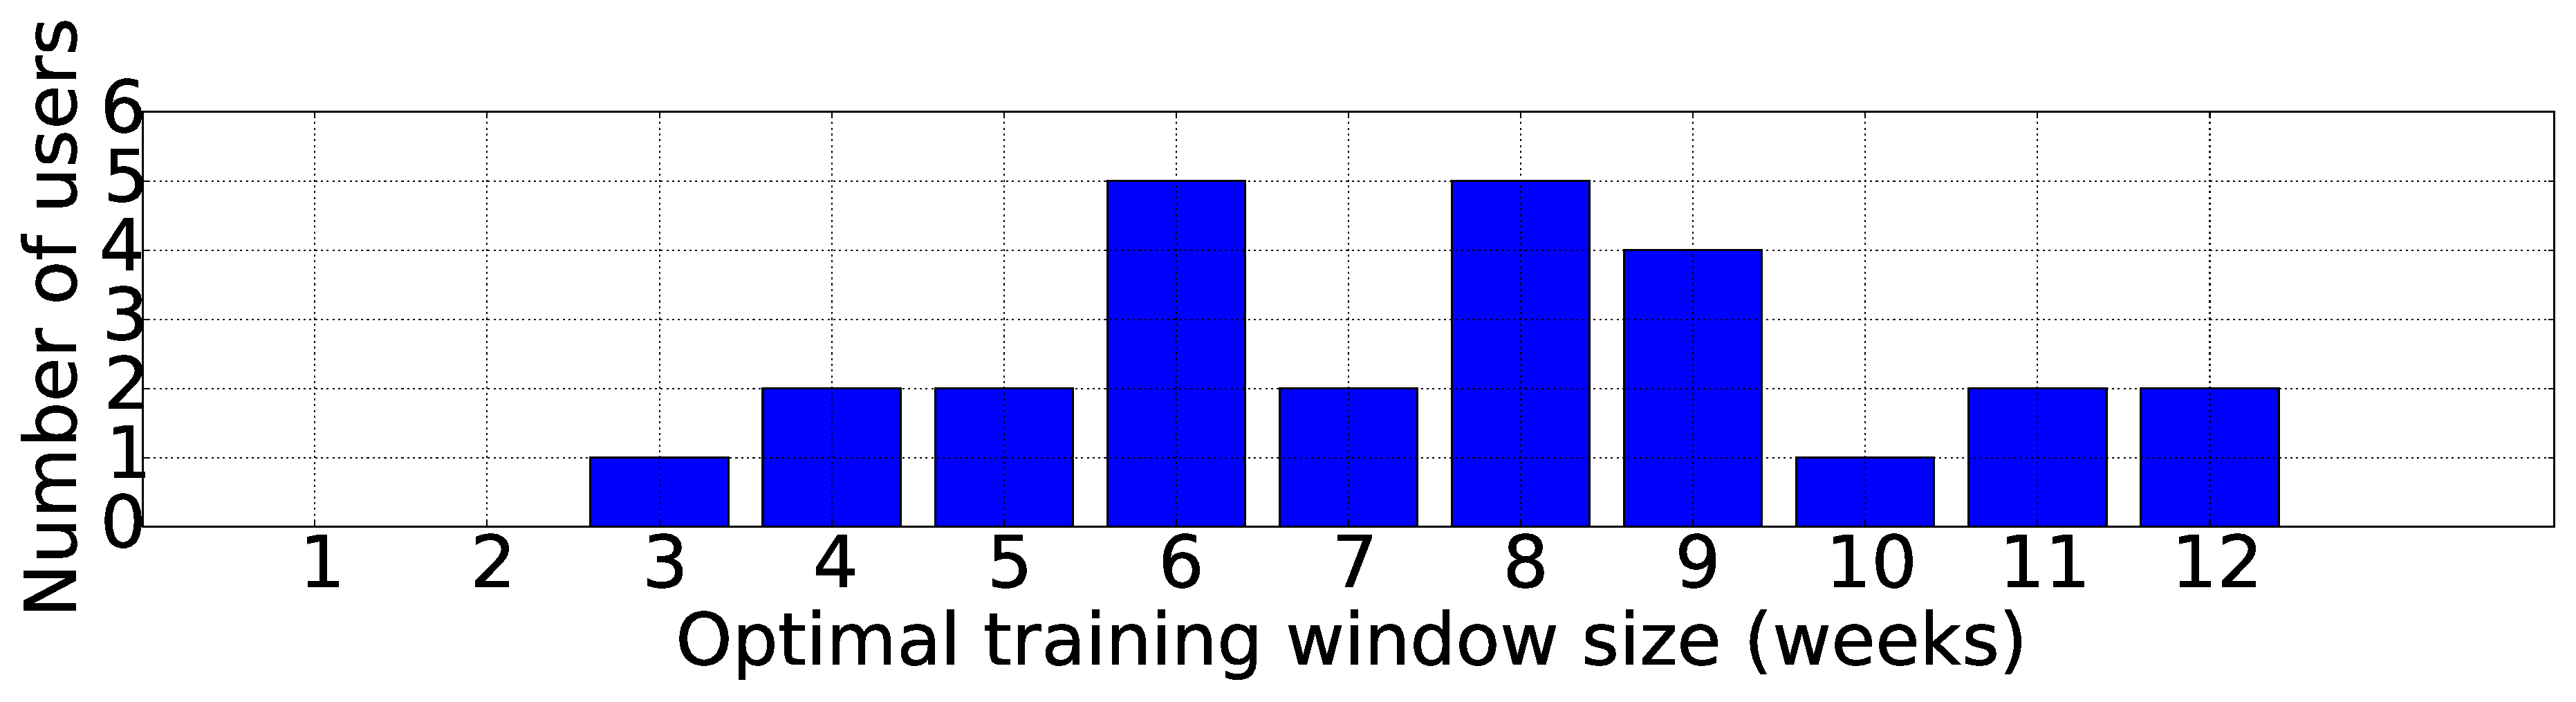
\includegraphics[width=0.95\linewidth]{FileAccess/figs/histogram_leastbestweekfscore6216New}
\caption{Distribution of the least number of weeks for each user of share D that gives highest F-score. } 
\label{fig:histBestLeastWeek6216}
\end{center}
%\vspace{-0.3in}
\end{figure}

Next, we perform a thorough study of the effect of training window
size on the performance of the models of individual users.  For this
purpose, we select share D, and divide its data into 17
parts, each corresponding to one week.  We remove 4 out of 30 users
because they do not have sufficient activity in each week.  We then
pick the last five weeks for the testing period, and create 12
different training windows, varying from 1 week to 12 weeks.  Based on
the results, we plot (Figure~\ref{fig:histBestLeastWeek6216}) the
distribution of the optimal training window size (in terms the least
number of weeks) providing the highest F-score for the evaluation
users of share D.  The median and the mode of this window is 8
weeks even though there are longer training windows up to 12 weeks,
thereby confirming our previous assertion that more training data does
not necessarily translate into better performance.  Additionally, we observe that
the optimal window size varies for each user.  The most active user
(with highest activity count) requires 4 weeks, whereas the least
active user requires 11 weeks.  This suggests that the optimal window
also depends on workload, with more active users requiring lesser
training time.

In a practical deployment, we could use an online evaluation approach
to continuously tune the system based on performance and workload
characteristics.  Lastly, it is important to note that some of the
recommended files, which are flagged as false positives in our
experiments, could in fact be true positives in an actual deployment
because users may genuinely find them useful.  Hence a precision
reported in this evaluation serves as the lower bound for the
precision expected from an actual deployment.


%% \indent We next study how the performance of the models of individual users varies for different training durations. In order to do so, we divide the data from share D on a weekly basis. Four out of 30 users do not have sufficient activity in each week and are hence removed in this analysis. For the same reason we have not provided these results for all eight shares. Figure~\ref{fig:histBestLeastWeek6216} shows the distribution of the least number of weeks that gives the highest F-score for evaluation users in share D. 
%% %\indent In order to analyze the performance variation of metadata models with finer time slices and on a per-user basis, 
%% %Only the training periods are varied 
%% For Figure~\ref{fig:histBestLeastWeek6216}, the test period comprises of the last five weeks to ensure that the 26 users have sufficient test data. 
%% The median and mode of the number of weeks giving highest F-score is seen to be 8 even though there are training periods that are 12 weeks long, showing that more training data need not improve the performance of a user model. It can be seen that the minimum size of training data required to give best F-score varies for each user. 
%% Due to space constraints, we are unable to provide complete statistics on activity rate of each user, and the performance variation of the user models. 
%% It is observed that while 4 weeks led to best performance for the most active user (in terms of the number of file activities in the share), the model corresponding to user with least activity required 11 weeks worth of training to provide best performance. This suggests that the optimal training duration differs for different users depending on their workloads. More active users typically need less number of weeks to collect sufficient activity to train a model that performs well. It is also seen that usually very small durations of training data do not lead to high performing models.

%% It must be mentioned that the entire performance evaluation of the system as described in this section is based on past activity. Upon actual deployment, the predictions can
%% be continuously compared with the actual accesses that users
%% make. This facilitates an online evaluation framework which can tune
%% the system parameters and adapt it based on the file edit rate, system performance and the
%% workload. For example using this framework, the size of training window and
%% frequency of re-training user models can be adjusted on a per-user basis to determine most
%% suitable values. In addition, as a result of the deployment of
%% the system, users would be able to discover files that they were
%% previously unaware of. It is possible that files that are considered
%% false positives by the evaluation framework presented in this paper, would be accessed
%% by users based on recommendations, and would hence be true positives
%% instead. Thus the precision reported in the current evaluation serves
%% as a lower bound for the precision expected upon actual deployment of
%% the system.
